%\documentclass[a4paper]{article}
\documentclass{apa6}
\usepackage[toc,page]{appendix}
\usepackage{apacite}
\usepackage[ruled,linesnumbered,vlined]{algorithm2e}
\usepackage{graphicx}

\title{Sneaky Thief}
\author{Stan Kerstjens\\ing. R.J.H.M Stevens\\Sina Maghami\\Rob Clinch\\Sharon Hallmanns}
\date{\today}
\affiliation{Department of Knowledge Engineering, \\Maastricht University}
\begin{document}
\maketitle
\section{Introduction}
% Problem Description
The posed problem is as follows. There is a world with two kind of people, guards and thieves. The guards have no greater goal than to catch the thieves, and the thieves have no larger purpose than to get to the valuables that they wish to acquire. The guards and thieves live on discrete tiles on a two dimensional game board among walls, doors, windows, and, of course, each other. This paper shall discuss various tasks both the guards and the guards in this world need to perform, and the appropriate algorithms to 

% Paper overview
	In the large, the problem  can be divided into three tasks. The first task is that guards put into an unknown environment should be able to create a 'mental map' of the environment. This is what we will call the exploration task. The second problem is that the guards should monitor the entire area as closely as possible to make it as difficult as possible for a possible intruder to pass through the area unseen. This will be called the coverage task. The third problem is that once an intruder has been detected, the guards should be able to actually catch the intruder. This will be called the pursuit task.

	In every of these three main problems the guard should figure out two things, namely where it should go, and how it gets there. The 'where'-question is largely dependent on the specific task at hand, e.g. even if an intruder would only be one unit of distance away, but the task is exploration, then the guard does not necessarily have to move towards the intruder.

	The 'how'-question, on the other hand, is in many cases independent of the exact task that we want to achieve, and therefore finding the shortest route to the destination does usually suffice, and is often even the best route. We will call the 'how'-question the pathfinding problem.

	The final task of the guards is to combine the three main problems and decide when the guard should solve what problem. The intuitive solution would be to explore until the entire environment is known, and then start, and continue, covering the area. During this process pursuit is started as soon as an intruder is detected. This intuitive answer, however, runs into issues once it is not known to the guard how big the area actually is, so it will never know if the map if fully explored or not. Another possible issue arises when an intruder, for instance, disappears behind a wall. The pursuing guard does not detect the intruder anymore and stops pursuit. He should, however, have the intelligence to predict where the guard has gone.
	
\section{Path finding}
		As already mentioned in the introduction, the answer to the question on what path to take to a certain location is in many cases not important as long as we find the shortest path. This is why we can first discuss general methods of path finding without referring to what goal the moving of the agents serves. There are also cases where the shortest path is not the best path. This is heavily dependent on the task, and will therefore be discussed in the sections dealing with the specific tasks.

    \subsection{A-star}
		%Introduction to A-star
			The A-star algorithm is a general purpose algorithm that searches a graph and is capable of providing the optimal path from one node to another. A-star is a heuristic search, and like many heuristic search algorithms its performance depends on the heuristic employed. Although A-star always finds the shortest path as long as the heuristic is admissible, i.e. the cost the heuristic estimates always underestimates the actual cost, a better heuristic will shorten the time needed to find this optimal path~\cite{hart1968}. The implemented instance of A-star uses Cartesian distance between the current and the goal tile as its heuristic, which is clearly admissible.

%Workings of A-star
			A-star uses an evaluation function $f(x)$ which depends on the cost function $g(x)$ and the heuristic function $h(x)$.
			\begin{equation}
				\label{eq:astarevaluation}
			 	f(x) = g(x) + h(x)
			\end{equation} 
			At every iteration it will expand the node that has the lowest cost as predicted by the evaluation function (see alg.~\ref{alg:astar}).

			\begin{algorithm}
				\KwData{Starting node $s$; Set of target nodes $T$; evaluation function $f$}
				Mark $s$ as 'open' and calculate $f(s)$\;
				\While{ There are open nodes left }{
    				Select the open node $n$ with the smallest $f$\;
    				\eIf{$n \in T$}{
    					Mark $n$ 'closed' and terminate\;
    				}{
    					Mark $n$ 'closed'\;
    					Let $A$ be the successors of $n$\;
    					\For{$a \in A$}{
    						Calculate $f(a)$\;
    						\If{$a$ is not closed $\vee f(a) < f$ when s was closed}{
    							Mark $a$ as open\;
    						}
    					}
    				}
				}
				\caption{A-star algorithm~\protect\cite{hart1968}}
				\label{alg:astar}
			\end{algorithm}

			In our simulations the nodes of the graphs will be simple coordinates, so for our heuristic function we can simply take the direct distance to the destination coordinate as our heuristic function.

			A disadvantage of the A-star algorithm in path finding is that it will not identify a certain coordinate as unreachable until all possible routes have failed. As this would take to long in most simulations to compute, it is necessary to provide a maximum amount of nodes the algorithm is allowed to explore before it has to give up the search. This, of course, is at the risk of falsely concluding that a certain position is unreachable.

			Another disadvantage of the A-star algorithm is that it is necessary to discretize the world in order for the algorithm to run. In real-world applications for robotic systems, most robots will not find themselves in a discrete world. Therefore the A-star algorithm will be very unlikely to find the optimal path in continuous world applications. If, however, the discretization is sufficiently narrow the proposed path will probably be sufficient for most purposes. Unfortunately, narrowing the discretization inherently leads to the need for more computing power.\cite{korf1990real, ASta2:online}

			\subsubsection{RTA-star}
				An adaptation of A-star to be more accommodating to real-time applications is Real-Time A-star (RTA-star). When the computational resources are insufficient to at every step recalculate the entire path from the agent to the goal, this method should be employed. It is very similar to regular A-star with the adaptation that an agent is immediately moved to the most promising direction, instead of first calculating the entire path. This way A-star loses its optimality, but it will execute a lot faster, which is necessary when computing long paths for many agents~\cite{korf1990real, rtastar, undeger2010multi, undeger2007single, undeger2009real}.

		
	\subsection{Reverse-A-star}
	Sometimes the best path is not simply defined by the shortest path towards a specific coordinate, but rather to avoid a certain coordinate. Our prey, for instance, wants to avoid the guards. To do this we can reverse the A-star algorithm, so instead of moving towards node with the highest

	\subsection{RTTE-h}
		
			The RTTE-h algorithm uses various geometrical features of the obstacles that the agent encounters to determine the best moving direction as an angle, and also the utilities of all discretised moving directions.

			%
			% Explain how RTTEh works
			%
			\begin{algorithm}[h!]
				\KwData{The agent's current cell $s$}
				\KwResult{Utilities of neighbours of $s$}
				Mark all moving directions of $s$ as open\;
				Propagate rays over the edges of the moving directions\;
				\For{each ray $r$ hitting an obstacle}{
					Let $o$ be the obstacle hit by $r$\;
					Extract border $b$ from $o$\;
					Detect closed directions of cell $s$ using $b$\;
					Extract geometric features of $o$\;
					Determine the best moving direction to avoid $o$\;
				}
				Merge the results (see alg.~\ref{alg:rrtehmerge})\;
				\Return utilities\;
				\label{alg:rtteh}
				\caption{RTTE-h algorithm~\protect\cite{undeger2010multi}}
			\end{algorithm}

			The merging phase of the algorithm determines the utilities as is described in alg.~2.


			\begin{algorithm}[h!]
				\KwData{current coordinate of the guard $s$; current coordinate of the target $t$; results from the rays $r$.}
				\If{All neighbours of $s$ are closed}{
					\Return failure\;
				}
				Determine most constraining obstacle $m$ from $r$\;
				\eIf{$m$ exists}{
					Let proposed direction $d$ be the direction that gets around $m$\;
				}{
					Let proposed direction $d$ be direct direction to $t$\;
				}
				\For{each neighbour $n$ of $s$}{
					\eIf{$n$ is closed}{
						Let utility of $n$ be $0$\;
					}{
						Let $dif$ be the smallest angle between $d$ and the direction of the cell $n$\;
						Let the utility of $n$ be $(181-dif)/181$\;
					}
				}
				\label{alg:rrtehmerge}
				\caption{Merging Phase of RTTE-h~\protect\cite{undeger2010multi}}
				\Return utilities\;
			\end{algorithm}

			The RTTEh alg.~6 provides answers to two shortcomings of the A* algorithm for path search. First, it is a continuous space algorithm, so it is not dependant on any kind of discretisation for real world applications. Second, it is capable of identifying whether a certain coordinate in space is unreachable without having to explore a large amount of possible routes.

			Another property that will be useful later on is that this algorithm returns an ordering of all moving directions, instead of just the best one.

			Although the algorithm operates in continuous space, the moving directions are still discretised. In real world applications this is usually not the case, and this will therefore lead to a suboptimal result.\cite{undeger2009real, undeger2010multi, undeger2007single}.

	\section{Exploration}

	\section{Coverage}
	Any intruder will try to be undetected. In order to increase the chance of detecting an intruder we need to make sure that the environment is monitored as closely as possible. This is the problem of coverage. Given the environment we want our agents so move in such a way that no intruder can move through the environment undetected. The intuitive answer behind this problem is to try to disperse the guards over the environment as well as possible, which is exactly what the StiCo algorithm aims to do.
	
		\subsection{StiCo}
			%TODO The caption and the image are from http://swarmlab.unimaas.nl/stico/stico-principle/ so there needs to be a reference to here

One way of covering the entire area of the environment is to try to equally disperse the guards over the area in a way that tries to cover as much of the area as possible. An algorithm that attempts to do this is the so called StiCo algorithm. In the StiCo algorithm all agents lay down a pheromone trail that other agents can detect. The principle is that once an agent detects a pheromone it changes its direction so to not cover an area that another agent already covers. In an non-open environment also the walls and other obstructions can be seen as these pheromones. In nature the pheromones are scents. In our world, the pheromones will be beacons dropped by the agent which can be seen by other agents \cite{ranjbar2012multi}.

The StiCo algorithm needs a base movement from which to start. This base movement is moving at a constant forward and angular velocity, which results into describing a circle (if not obstructed). Any time the agent encounters a pheromone trail, it simply changes its angular velocity to move another direction. To determine what direction is the best one to avoid the pheromone trail the agent has two different sensors: an interior, and an exterior. The interior sensor is the one on the inside of the circular motion, and the exterior one is the one on the outside of the circular motion described by the agent. If the interior sensor picks up the pheromone trail, the easiest way to avoid the pheromones is to invert the angular velocity. If the exterior sensor picks up the pheromone trail the agent should temporarily increase its angular velocity to avoid the pheromone trail (see alg. \ref{alg:StiCo}, fig. \ref{fig:movingDirections})~\cite{ranjbar2012multi}.

\begin{algorithm}
\label{alg:StiCo}
\caption{Iteration of the StiCo Algorithm~\protect\cite{ranjbar2012multi}}
	\While{no pheromone encountered}{
		Move with velocity $v$ and angular velocity $a$\;
	}
	\eIf{Encountered pheromone at interior sensor}{
		$a\leftarrow -a$\;
	}{
		\While{Pheromone is detected}{
			increase $a$\;
		}
		Set $a$ back to the original value\;
	}
\end{algorithm}

\begin{figure}
\centering
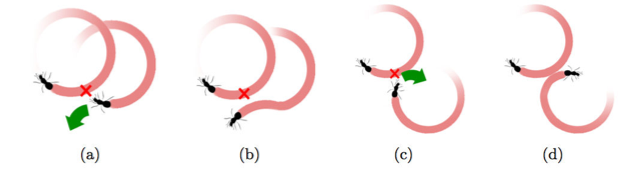
\includegraphics[width=\columnwidth]{images/stico.png}
\caption{StiCo coordination principle (a) and (c) before pheromone detection (b) and (d) after pheromone detection~\protect\cite{ranjbar2012multi}}
\label{fig:movingDirections}
\end{figure}

A great advantage of the StiCo algorithm, apart from its simplicity, is that no prior map of the environment is needed. Therefore, we can skip the entire exploration phase and not bother with trying to figure out when exactly an agent should explore the environment, and when it should cover the known map. Also there is no initial time the agent needs to spend exploring.

The other side of the coin is that the agent also does not use a map of the environment. It does not intelligently cope with features of the environment such as entries, doors, windows, exits, sentry towers, etc.

Moreover, the algorithm often reaches an equilibrium, namely when no territories, the area described by the circular motion of an agent, of the agents intersect. There, however, is no guarantee that this equilibrium covers the entire area. One could argue that if this is the case, there are simply not a sufficient amount of guards guarding the premise, but it is quite obvious that in a mansion with only one guard, the guard should not just stand in the main hall walking circles, hoping to run into an intruder.

% the source of this text is http://swarmlab.unimaas.nl/stico/stico-principle/

	\section{Pursuit}
		When considering the problem of pursuit, there is again a very simple intuitive answer, namely to go directly to the location of the intruder following the shortest path. This will often be the best solution if you are a lone guard pursuing an intruder. Yet even then, this strategy will only work if either the intruder is not actively avoiding the guard, or the guard is faster than the intruder. As we are not prepared to assume any of these conditions, we need to act slightly more intelligently.

	    \subsection{MTES}
			The Real-time Moving Target Evaluation Search (MTES) is an assisting algorithm that prevents an agent in retracing it steps. The concept is very simple: every visited cell is considered as an obstable, until the target becomes unreachable through visited cells. At this point it will clear the history and start over.

			In a static environment where the target of the path search does not change there is a very low risk that an algorithm searching for the shortest path will ever try to visit the same cell twice. When the target moves, however, a path-finding algorithm might be advised to just go back and forth, which is undesirable.

			An example where this history could help is when two guards are pursuing an intruder around an obstacle. If the shortest path to the intruder is always chosen, the intruder and guards will continue to walk circles around the obstacle. If the guard, however, holds a record of where he's already been, he will try alternative paths as soon as one cycle has been made.

			This assisting algorithm requires the use of another path finding algorithm. The RTTE-h algorithm particularly suitable, since it does not only recommend a single moving direction, but multiple. If the first moving direction is blocked by a history cell, MTES can just select the second recommendation (see alg.~\ref{alg:mtes}).

			\begin{algorithm}[H]
				\KwData{Current cell $s$}
				Let $d$ be the proposed direction as determined by RTTE-h\;
				\eIf{$d$ exists}{
					Let $n$ be the neighbour cells of $s$ with minimum visit count\;
					Let $c$ be the cell in $n$ with maximum utility\;
					Move to $c$\;
					Increment the visit count of $s$\;
					Insert $s$ into history\;
				}{
					\eIf{History is not empty}{
						Clear history\;
						Go to next iteration\;
					}{
						Stop search with failure\;
					}
				}
				\label{alg:mtes}
				\caption{Iteration of MTES~\protect\cite{undeger2010multi}}
			\end{algorithm}

		\subsection{Blocking Escape Directions}
			A possible way of catching an intruder that is faster than the guards is to use the fact that there multiple guards pursuing a single intruder. In this case the guards should surround the intruder as much as possible, as to block all the possible direction in which he could escape. Then the guards can draw in and catch the intruder. The most naive way of doing this is to disperse the available guards equally amongst the circumference of an intruder. The guard closest to the intruder will always move directly towards the intruder following the shortest path. The other guards will establish the amount of pursuing guards ($n$) and each block one of the angles resulting from dividing the total angle in which the agent can move in equal parts ($2\pi / n$).

			%
			% Insert explanatory graphics
			%

			\begin{algorithm}
			\KwData{The guard $p$; the current cell of the guard $s$; the current cell of the intruder $t$; the number of guards $n$}
			\KwResult{Blocking location}
			Let $(h_x,h_y)$ be the coordinate of cell $s$\;
			Let $(t_x,t_y)$ be the coordinate of cell $t$\;
			\eIf{ $n = 1$ or $p$ is the nearest guard to $t$}{
				\Return $(t_x,t_y)$\;
			}{
				Calculate the set of escape directions $e$\;
				Determine the map $m$ that maps the guard to $e$ optimally\;
				Let $esc$ be the escape direction assigned to $p$ in $m$\;
				\Return the blocking location using $esc$ (alg.~\ref{alg:calcblockloc}) \;
			}
			\label{alg:blockloc}
			\caption{Determining the Blocking Location}
			\end{algorithm}

			To exactly calculate the blocking location in the last step of algorithm \ref{alg:blockloc} we execute algorithm~\ref{alg:calcblockloc}.

			\begin{algorithm}
				\KwData{the guard $p$; the velocity of the guard $v_h$; the velocity of the intruder $v_p$; the escape direction $es$assigned to $p$}
				Let $\epsilon$ be a small number (0.5)\;
				Let $\varepsilon$ be a very small number(0.05)\; 
				Let $\alpha$ be the smallest angle between $es$ and the direction from $p$ to the intruder\;
				Let $d_{max}$ be the maximum permitted distance between the blocking location and the intruder\;
				\eIf{$\epsilon < \alpha < 180 -\epsilon$}{
					\eIf{$(\sin\alpha)(1+\epsilon)(v_p/v_h)\leq 1$}{
						Let $\theta$ be $\arcsin((\sin\alpha)(1+\varepsilon)(v_p/v_h))$
						\eIf{$\theta < 180 - \alpha - \epsilon$}{
							Let $pdir$ be the guard direction using $\theta$\;
							Let $bl$ be the intersection point of lines passing through $es$ and $pdir$\;
							\eIf{Distance between $bl$ and the intruder $> d_{max}$}{
								\Return the point with distance $d_max$ from the intruder in the direction of $es$\;
							}{
								\Return bl\;
							}
						}{
							\Return the point with distance $d_max$ from the intruder in the direction of $es$\;
						} 
					}{
						\Return the point with distance $d_max$ from the intruder in the direction of $es$\;
					}
				}{
					\Return the location of the intruder\;
				}
				\label{alg:calcblockloc}
				\caption{Calculating the Blocking Location}
			\end{algorithm}


	\section{Simulator environment}
		\subsection{Time perception}
			The time in the simulator is perceived continuouly to allow for continuous velocity, even in a discretized world. Although the moves of the agents on the map are fully discretized, the simulator takes into account how long this unit move has taken to perform, and only allows the same agent to move again once all other agents have caught up with his 'time'. In other words, each agent has his own progress in time, and is only allowed to move when his time is lower (or equal) than all the other agents.
		\subsection{Game Rules}



\section{Results}
	% This chapter should contain all experimental results that we obtain (lots of graphs!)
	
\section{Discussion}


\chapter{Conclusions}
	% This chapter should contain all our conclusions of how the experimental results compare to our initial expectations.
	% Also it should contain our evaluation of the different approaches we took towards the problems

\bibliographystyle{apacite}
\bibliography{references.bib}
% All references APA style

\begin{appendices}
\section{Other Data}
	
\end{appendices}



\end{document}
